\documentclass[aspectratio=169]{beamer}
\usetheme{default}
\usepackage{amsmath,amssymb,braket,graphicx,booktabs}

\title{Quantum numerical linear algebra}
\author{Dong An}
\institute{Beijing International Center for Mathematical Research, Peking University\\
\texttt{dongan@pku.edu.cn}}
\date{April 11, 2026}

\begin{document}

\begin{frame}\titlepage\end{frame}

\begin{frame}{Overview}
\begin{itemize}
\item Introduction to quantum computing
\item Basic linear algebra operations
\item Matrix functions
\item Application: Hamiltonian simulation
\item Application: Linear systems of equations
\item Summary
\end{itemize}
\end{frame}

\section{Introduction to quantum computing}
\begin{frame}\sectionpage\end{frame}

\begin{frame}{Quantum computing}
\begin{quote}
``If you want to make a simulation of nature, you'd better make it quantum mechanical, and by golly it's a wonderful problem, because it doesn't look so easy.'' [Feynman (1982)]
\end{quote}
\begin{itemize}
\item Using the nature of quantum mechanics to perform computing
\item Quantum advantage:
\begin{itemize}
\item Unstructured search: Quantum cost $O(\sqrt{N})$ vs.\ Classical cost $O(N)$
\item Fourier transform: Quantum cost $O((\log N)^2)$ vs.\ Classical cost $O(N\log N)$
\end{itemize}
\end{itemize}
\end{frame}

\begin{frame}{Quantum algorithm hierarchy}
\centering
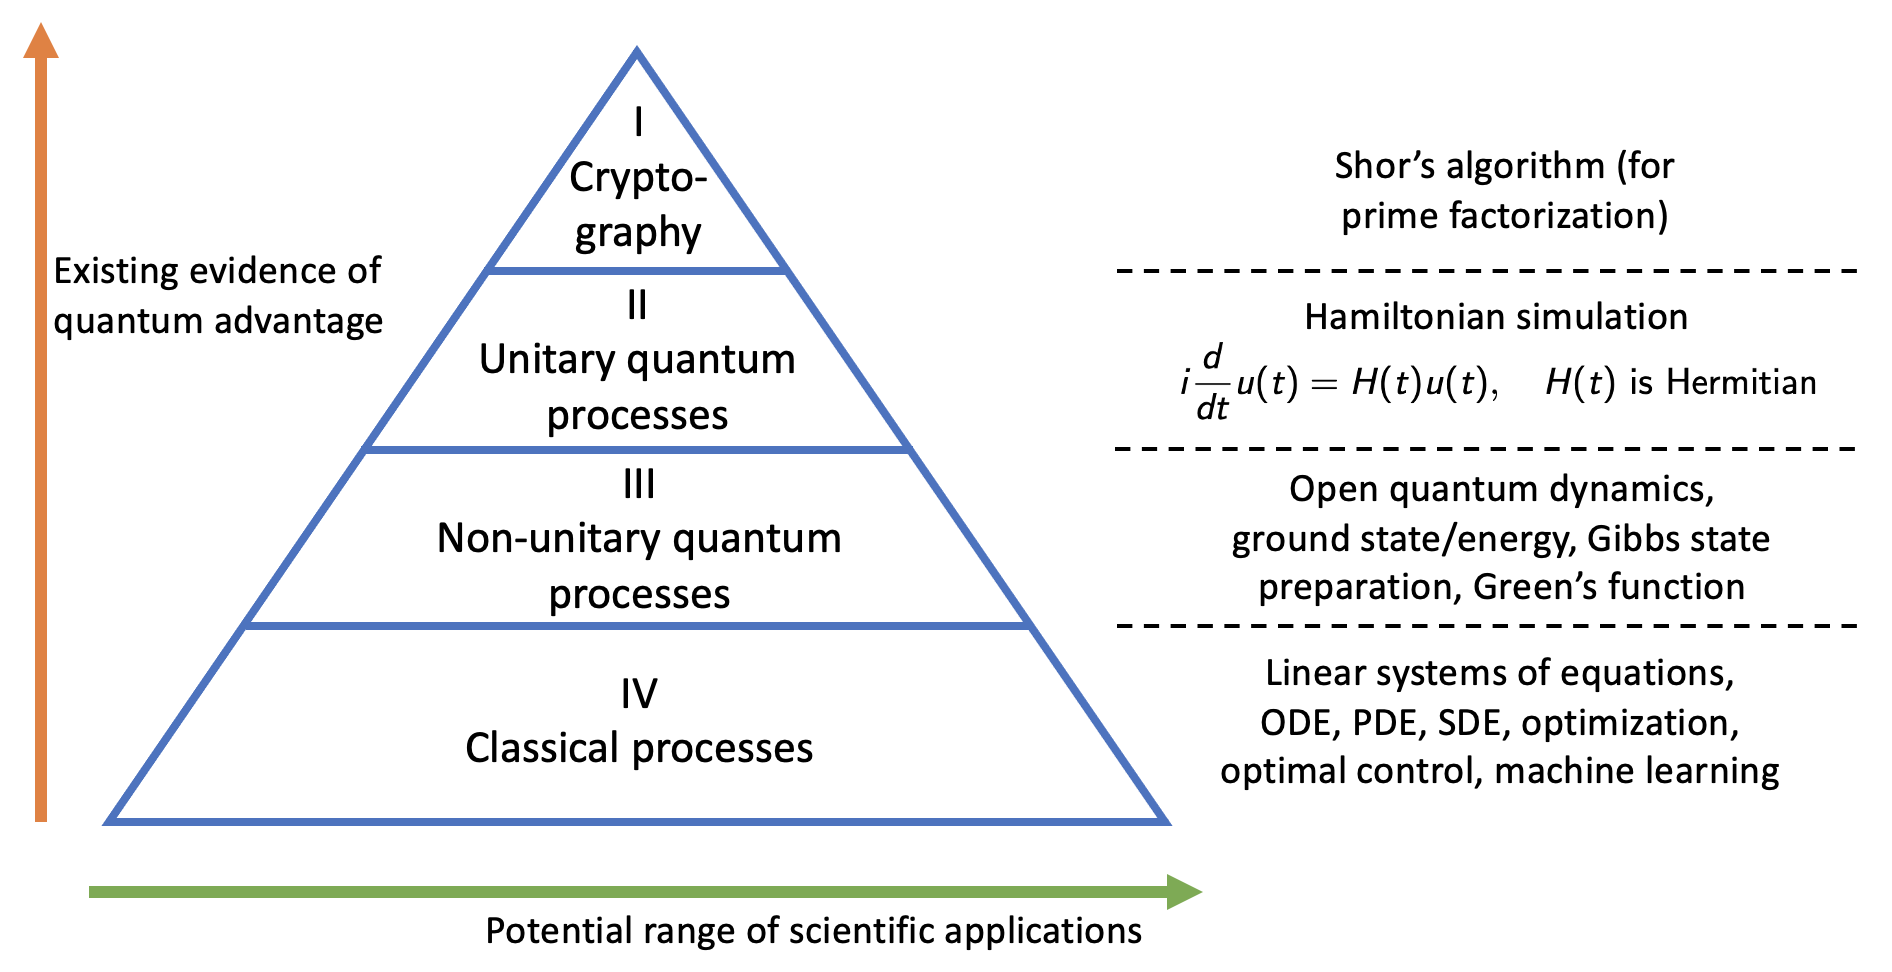
\includegraphics[width=0.85\textwidth]{images/page_5_img_1.png}
\footnotetext{Adapted from [Lin Lin. Lecture Notes on Quantum Algorithms for Scientific Computation]}
\end{frame}

\begin{frame}{Quantum algorithm flow map}
\centering
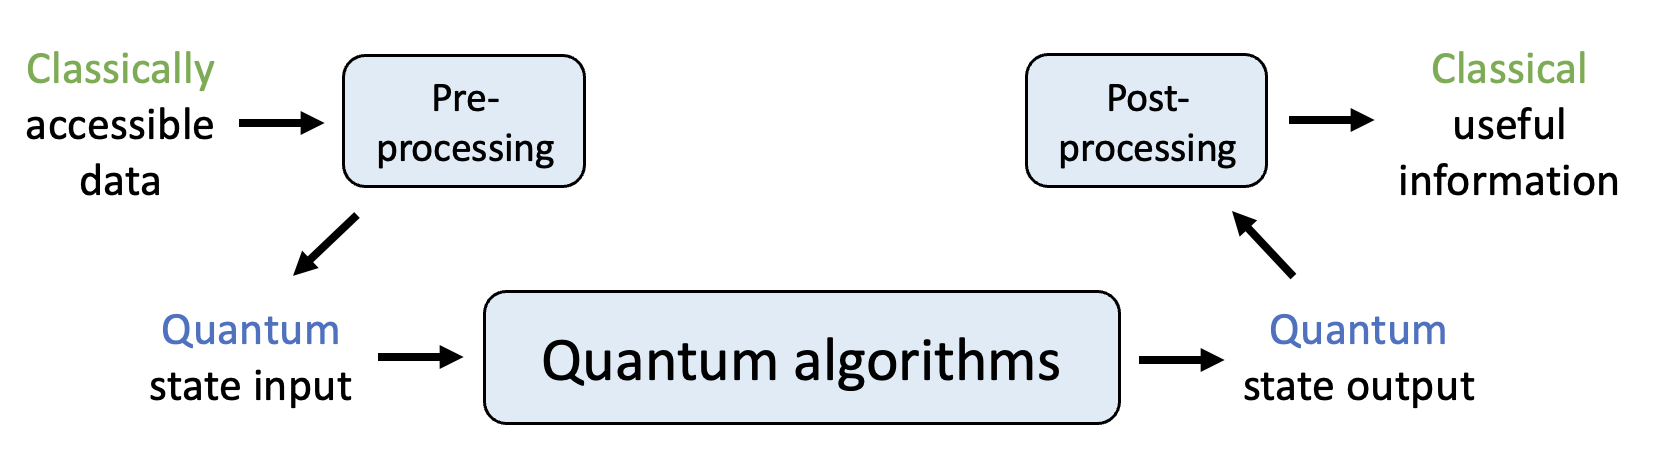
\includegraphics[width=0.92\textwidth]{images/page_6_img_1.png}
\end{frame}

\begin{frame}{Input: quantum states}
\textbf{A qubit (quantum bit):} $\mathbb{C}^2$
\begin{itemize}
\item Instead of 0 or 1, quantum allows superposition $\alpha\ket{0}+\beta\ket{1}$
\item Measurement: get 0 with prob $|\alpha|^2$, get 1 with prob $|\beta|^2$
\item Orthonormal basis $\ket{0}=(1,0)^T$, $\ket{1}=(0,1)^T$
\end{itemize}
\textbf{Multi-qubit system:} $\mathbb{C}^{2^n}$, $N=2^n$
\begin{itemize}
\item Superposition of $2^n$ possible states $\ket{j}$, $0\le j\le 2^n-1$:
$$\ket{u}=\sum_{j=0}^{2^n-1}\alpha_j\ket{j}\cong(\alpha_0,\alpha_1,\ldots,\alpha_{2^n-1})^T$$
\item Tensor product: $\ket{u}=\ket{u_A}\otimes\ket{u_B}=\ket{u_A}\ket{u_B}$
\end{itemize}
\end{frame}

\begin{frame}{Input: quantum states}
\textbf{Dirac notations:}
\begin{itemize}
\item $\ket{u}=(\alpha_0,\ldots,\alpha_{N-1})^T\in\mathbb{C}^N$, $\|\ket{u}\|=1$
\item Computational basis: $\{\ket{j}\}_{j=0}^{N-1}$, \quad $\ket{u}=\sum_{j=0}^{N-1}\alpha_j\ket{j}$
\item $\bra{u}=\ket{u}^\dagger$
\item Inner product: $\braket{u|v}$
\item Observable: $\bra{u}O\ket{u}$
\end{itemize}
\end{frame}

\begin{frame}{Quantum algorithms}
\textbf{Quantum algorithms:} Implement a series of unitary transformations
$$U_K\cdots U_2 U_1\ket{\psi_{\mathrm{in}}}=\ket{\psi_{\mathrm{out}}}$$
\begin{itemize}
\item A quantum version of numerical linear algebra
\end{itemize}
\end{frame}

\begin{frame}{Post-processing}
$$\ket{u}=\sum_{j=0}^{N-1}\alpha_j\ket{j}$$
\textbf{Measurement:} collapse to $\ket{j}$ with probability $|\alpha_j|^2$
\begin{itemize}
\item Extract amplitude info or more general $\bra{u}O\ket{u}$
\item Post-select on ``good subspace'':
$\ket{\psi}=\sqrt{p}\ket{0}\ket{\psi_{\mathrm{out}}}+\sqrt{1-p}\ket{\mathrm{bad}}$;
expected repeats $O(1/p)$
\item \textbf{Amplitude amplification (AA):} apply reflections, then measure;
expected repeats $O(1/\sqrt{p})$
\end{itemize}
\end{frame}

\begin{frame}{Complexity and quantum circuits}
\textbf{Quantum complexity:}
\begin{itemize}
\item Query complexity: number of oracle calls
\item Circuit depth: number of coherent layers
\end{itemize}
\textbf{Quantum circuits:} graphical representation
$$\ket{1}\ \xrightarrow{e^{i\tilde\phi_d Z}}\ \cdots\ \xrightarrow{e^{i\tilde\phi_0 Z}}$$
$$\ket{0}\ \xrightarrow{U_A}\ \xrightarrow{U_A^\dagger}\ \cdots\ \xrightarrow{U_A^{(\dagger)}}$$
$$\ket{u}\ \cdots$$
\end{frame}

\section{Basic linear algebra operations}
\begin{frame}\sectionpage\end{frame}

\begin{frame}{Input model: vectors}
\textbf{State preparation oracle:}
$$O_u:\ket{0}\to\ket{u}=\sum_{j=0}^{2^n-1}u_j\ket{j}$$
Constructing $O_u$ is generally hard, but efficient in special cases.\footnote{[arXiv:quant-ph/0208112], [arXiv:2201.11495]}
\end{frame}

\begin{frame}{Input model: matrices}
\begin{block}{Definition (Block-encoding)}
Let $A$ be $2^n\times 2^n$. A \textbf{block-encoding} of $A$ is a $2^{n+a}\times 2^{n+a}$ unitary $U_A$ such that
$$A\approx\alpha\bigl(\bra{0}^{\otimes a}\otimes I\bigr)U_A\bigl(\ket{0}^{\otimes a}\otimes I\bigr),
\quad\text{i.e.,}\quad
U_A\approx\begin{pmatrix}\tfrac{1}{\alpha}A & * \\ * & *\end{pmatrix}.$$
\end{block}
\begin{itemize}
\item $\alpha\ge\|A\|$ is the block-encoding factor
\item Serves as both input and output model
\end{itemize}
\end{frame}

\begin{frame}{Input model: matrices}
$$U_A\approx\begin{pmatrix}\tfrac{1}{\alpha}A & * \\ * & *\end{pmatrix}$$
\begin{itemize}
\item Constructing $U_A$ for arbitrary $A$ is in general hard
\item Special cases: unitary, sparse, structured matrices, \ldots\footnote{[arXiv:1806.01838], [arXiv:2203.10236]}
\end{itemize}
\end{frame}

\begin{frame}{Matrix-vector multiplication}
\centering
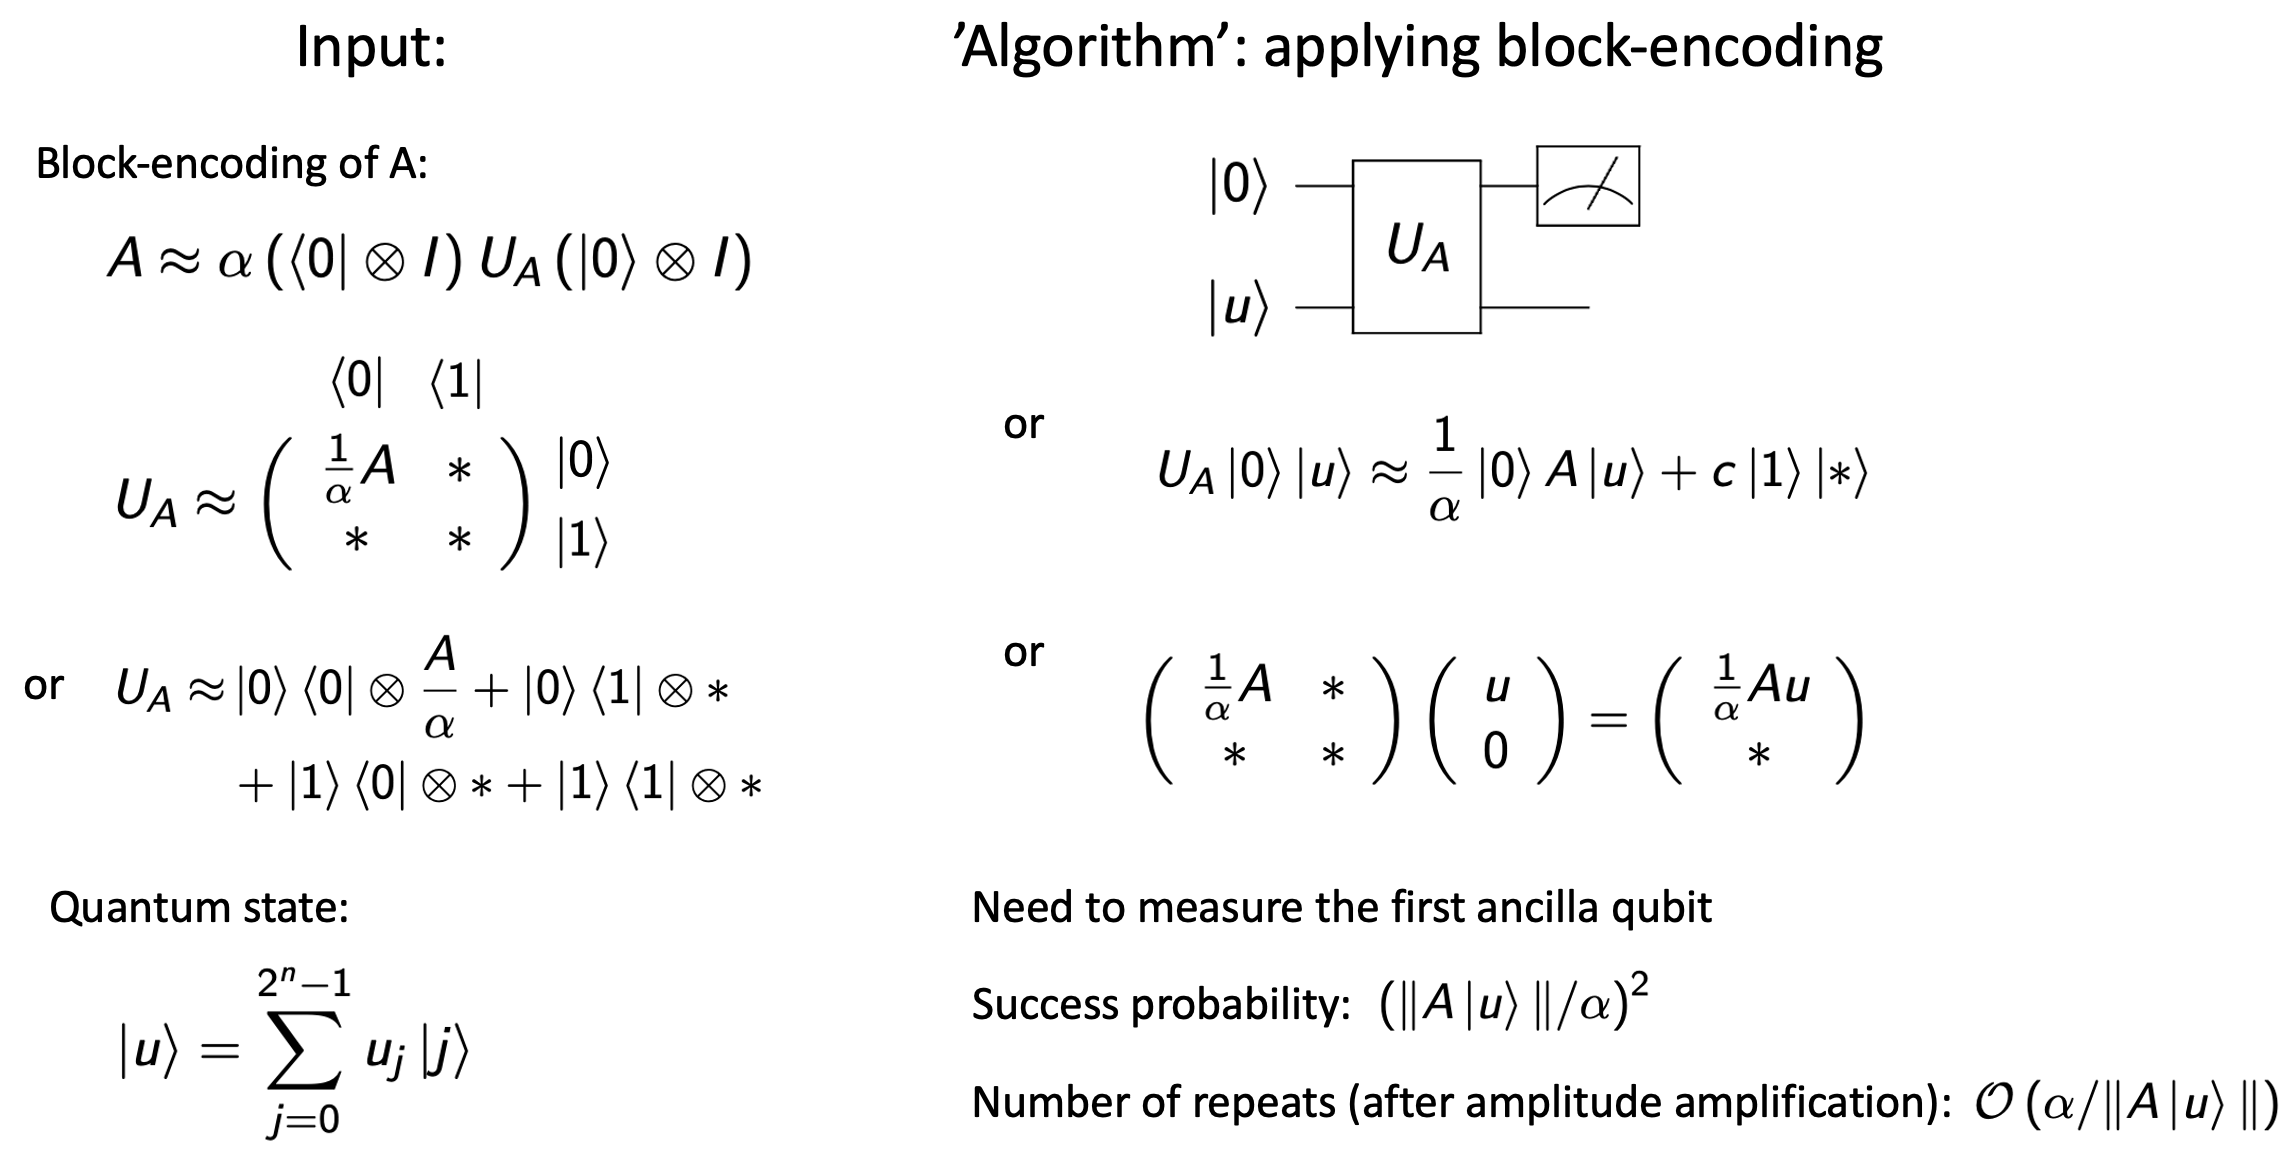
\includegraphics[width=0.92\textwidth]{images/page_16_img_1.png}
\end{frame}

\begin{frame}{Matrix addition: Linear combination of unitaries (LCU)}
\textbf{Task:} given unitaries $\{U_j\}$ and $c_j\in\mathbb{R}_+$, compute $\sum_j c_j U_j$
\begin{itemize}
\item General matrix addition: $U_j$'s are block-encodings
\item Vector addition: $U_j$'s are state preparation oracles
\end{itemize}
\end{frame}

\begin{frame}{Matrix addition: LCU}
\centering
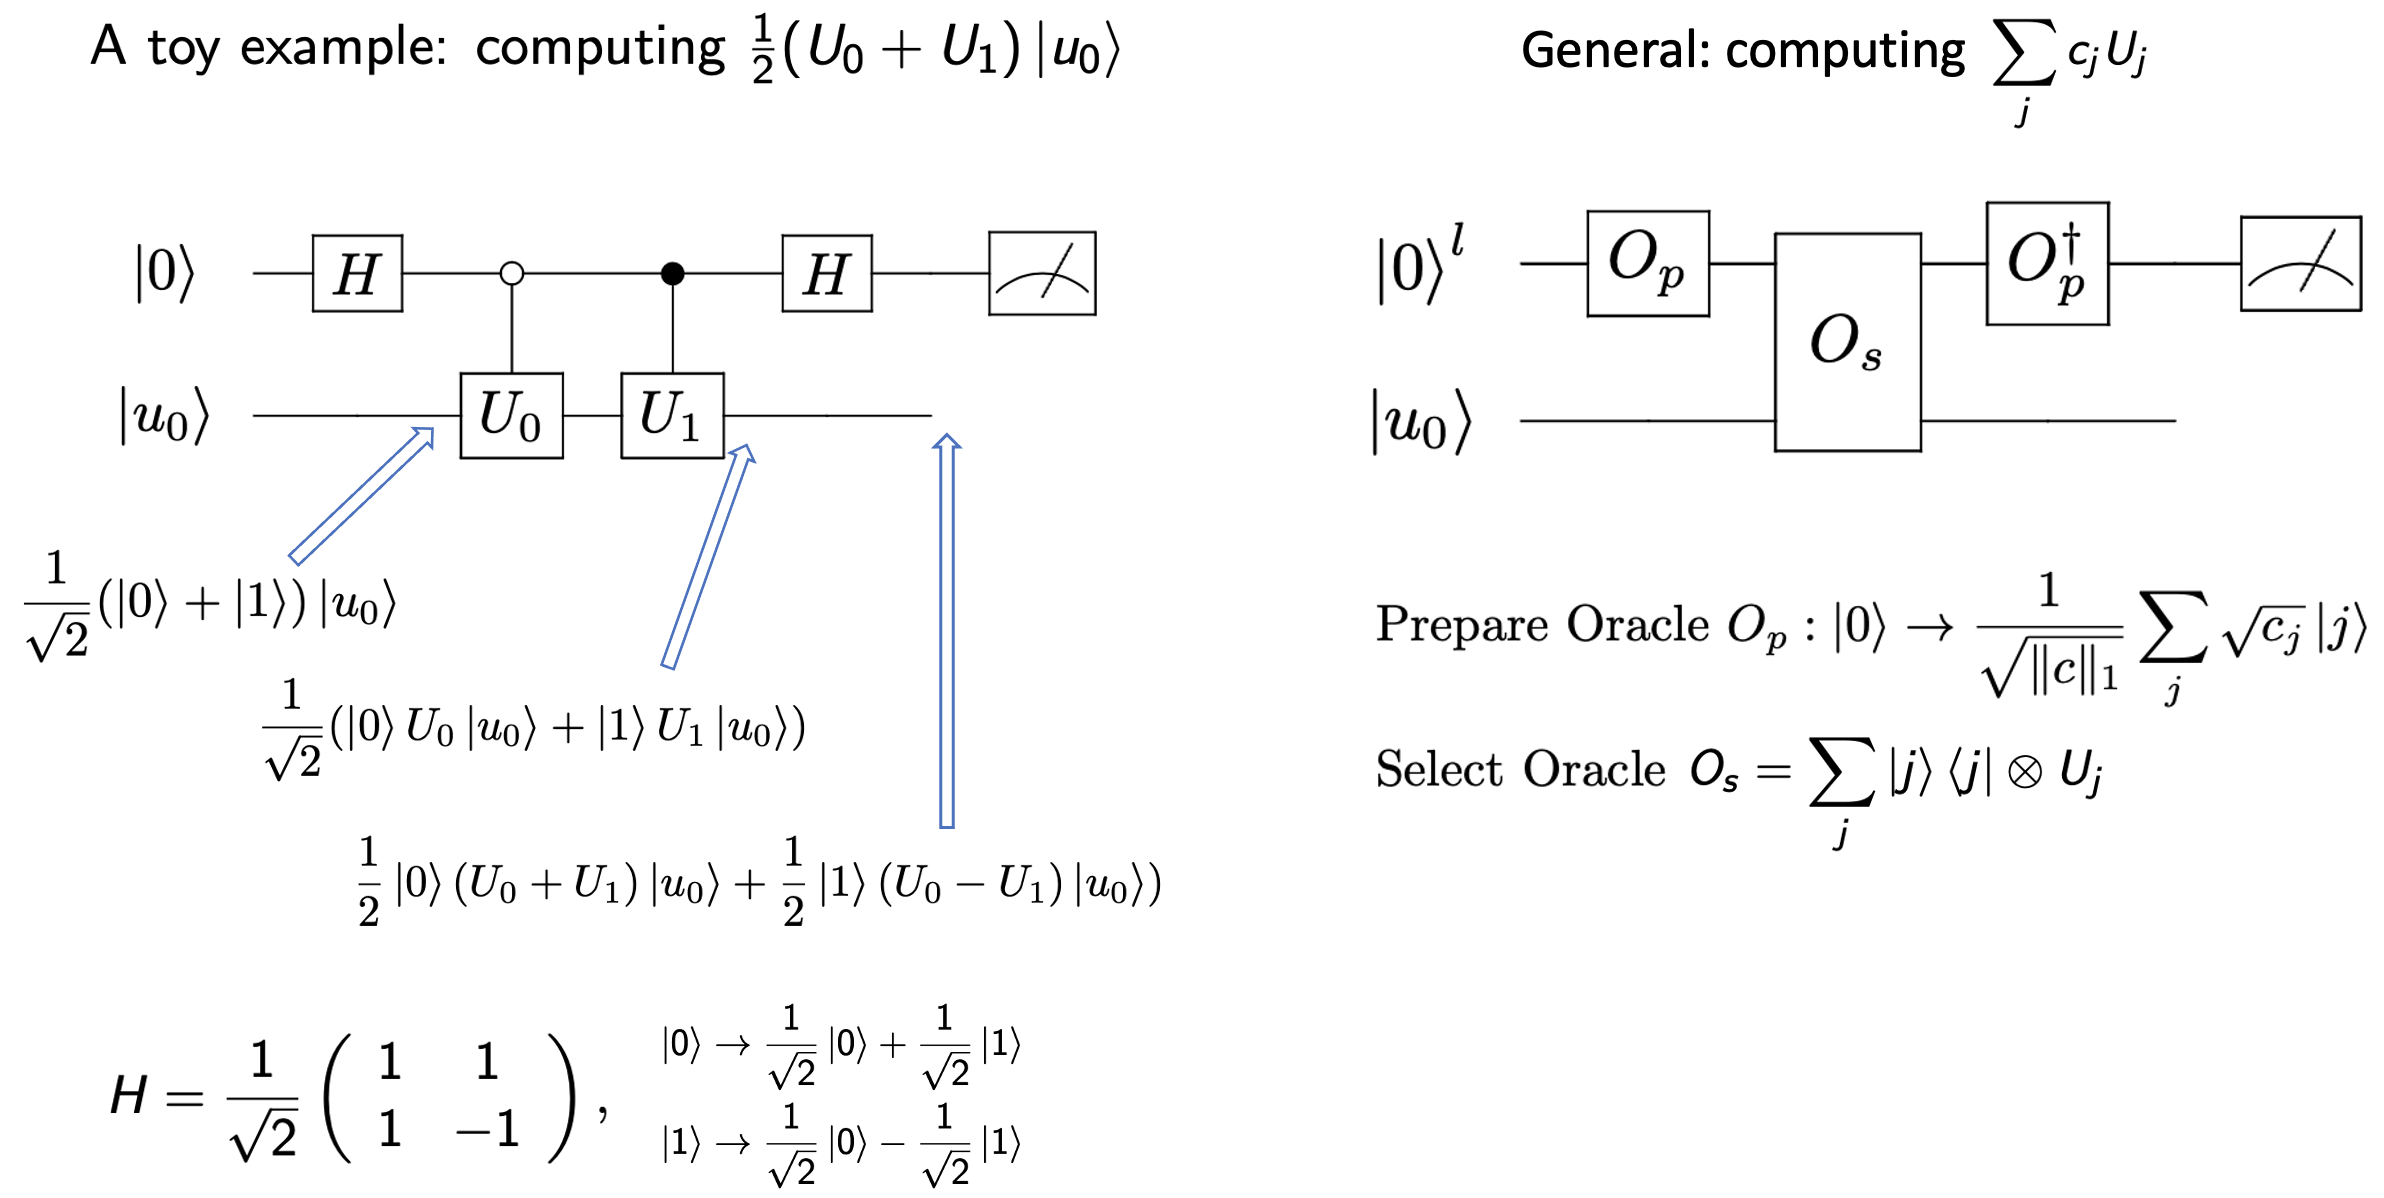
\includegraphics[width=0.85\textwidth]{images/page_18_img_1.png}
\end{frame}

\begin{frame}{Matrix addition: LCU}
\begin{columns}
\begin{column}{0.55\textwidth}
\small
\begin{align*}
\ket{0}\ket{u_0}&\xrightarrow{O_p}\tfrac{1}{\sqrt{\|c\|_1}}\sum_j\sqrt{c_j}\ket{j}\ket{u_0}\\
&\xrightarrow{O_s}\tfrac{1}{\sqrt{\|c\|_1}}\sum_j\sqrt{c_j}\ket{j}U_j\ket{u_0}\\
&\xrightarrow{O_p^\dagger}\tfrac{1}{\|c\|_1}\ket{0}\sum_j c_jU_j\ket{u_0}+\ket{\perp}
\end{align*}
\begin{itemize}
\item Repeats: $O\!\left(\|c\|_1/\|\sum_j c_jU_j\ket{u_0}\|\right)$
\item Cost depends on constructing $O_p$, $O_s$
\end{itemize}
\end{column}
\begin{column}{0.42\textwidth}
\centering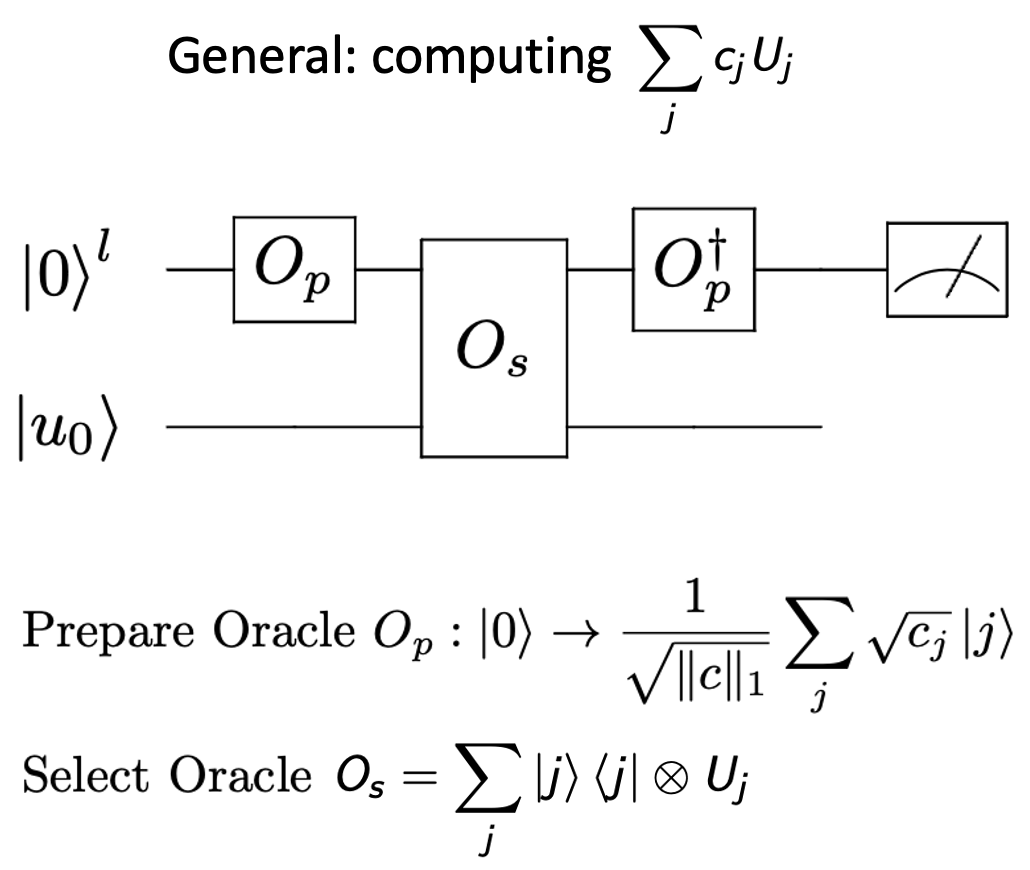
\includegraphics[width=\textwidth]{images/page_19_img_1.png}
\end{column}
\end{columns}
\end{frame}

\begin{frame}{Hybrid implementation of LCU: Importance sampling}
\begin{columns}
\begin{column}{0.55\textwidth}
$$u=\sum_j c_jU_j\ket{u_0}$$
$$\Rightarrow u^\dagger Ou=\sum_{j,j'}c_jc_{j'}\bra{u_0}U_j^\dagger OU_{j'}\ket{u_0}$$
\end{column}
\begin{column}{0.42\textwidth}
\centering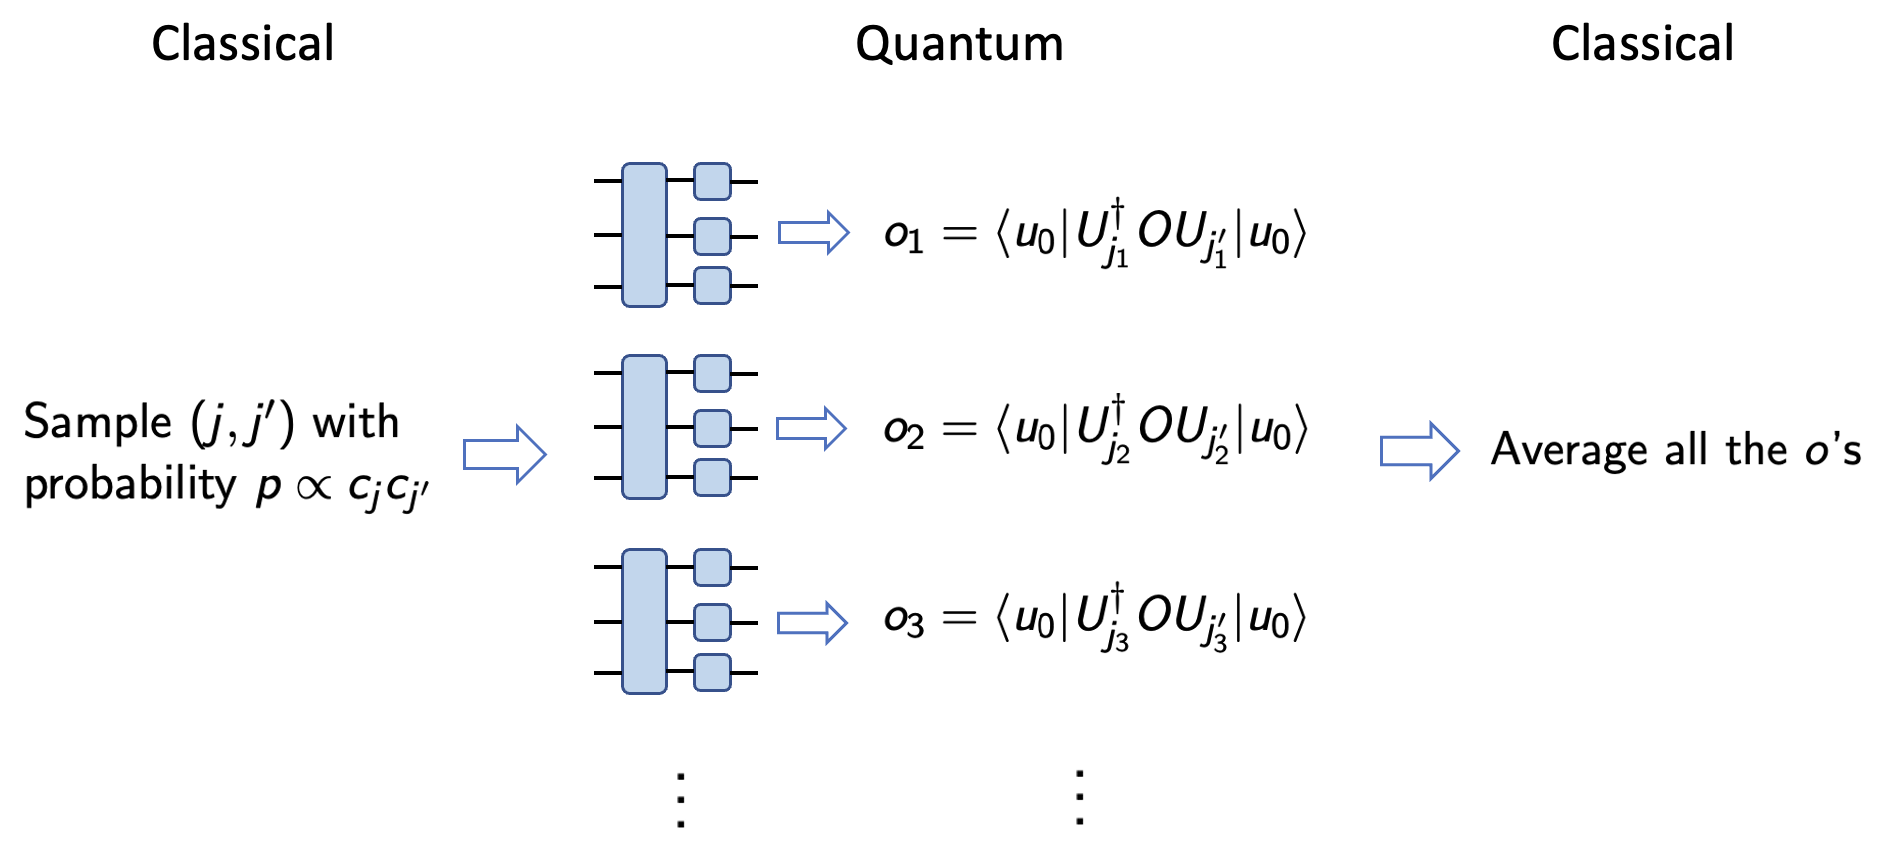
\includegraphics[width=\textwidth]{images/page_20_img_1.png}
\end{column}
\end{columns}
\end{frame}

\begin{frame}{Summary of basic linear algebra operations}
\textbf{Input models:} Vector: quantum state \quad Matrix: block-encoding\\[6pt]
\textbf{Algorithms:}
\begin{itemize}
\item Matrix-vector multiplication
\item Matrix/vector addition: LCU
\end{itemize}
\textbf{Other algorithms (not covered today):}
\begin{itemize}
\item Inner product/observable: SWAP test, Hadamard test
\item Matrix multiplication
\end{itemize}
Reference: [Section 4, arXiv:1806.01838]
\end{frame}

\section{Matrix functions}
\begin{frame}\sectionpage\end{frame}

\begin{frame}{Matrix functions}
\begin{itemize}
\item For Hermitian matrices: eigenvalue transformation
$$A=V\mathrm{diag}(\lambda_j)V^\dagger\ \longrightarrow\ f(A)=V\mathrm{diag}(f(\lambda_j))V^\dagger$$
\item For general matrices: singular value transformation
$$A=W\mathrm{diag}(\sigma_j)V^\dagger\ \longrightarrow\ f(A)=W\mathrm{diag}(f(\sigma_j))V^\dagger$$
or $\longrightarrow V\mathrm{diag}(f(\sigma_j))V^\dagger$ or $\longrightarrow W\mathrm{diag}(f(\sigma_j))W^\dagger$
\end{itemize}
\end{frame}

\begin{frame}{Main result}
Suppose $U_A$ block-encodes Hermitian $A$ with $\|A\|\le 1$, and $p(x)$ is a real polynomial s.t.\
\begin{enumerate}
\item $\deg(p)=d$,
\item $|p(x)|\le 1$ for all $x\in[-1,1]$.
\end{enumerate}
Then $p(A)$ can be block-encoded with complexity $O(d)$.\footnote{Gily\'{e}n et al.\ [arXiv:1806.01838]}
\end{frame}

\begin{frame}{Applications}
\begin{itemize}
\item Linear systems: $f(x)=1/(\kappa x)$
\item Hamiltonian simulation: $f(x)=e^{-ixt}$
\item Filtering
\item Amplitude amplification: $U\ket{0}\ket{\psi}=\frac{1}{q}\ket{0}A\ket{\psi}+\ket{\perp}$
$\to\tilde{U}\ket{0}\ket{\psi}=\frac{1}{2}\ket{0}A\ket{\psi}+\ket{\perp}$,\quad
$f(x)=qx/2$, $\deg(p)\sim q\log(1/\epsilon)$
\item $\cdots$
\end{itemize}
\end{frame}

\begin{frame}{Toy example: Chebyshev polynomials}
$$T_0(x)=1,\quad T_1(x)=x,\quad T_{k+1}(x)=2xT_k(x)-T_{k-1}(x),\quad T_k(\cos\theta)=\cos(k\theta)$$
\end{frame}

\begin{frame}{Toy example: Chebyshev polynomials}
Consider $2\times 2$ matrices (let $\theta=\arccos\lambda$):
$$U(\lambda)=\begin{pmatrix}\lambda&\sqrt{1-\lambda^2}\\\sqrt{1-\lambda^2}&-\lambda\end{pmatrix},\quad
Z=\begin{pmatrix}1&0\\0&-1\end{pmatrix},\quad
O=U(\lambda)Z=\begin{pmatrix}\cos\theta&-\sin\theta\\\sin\theta&\cos\theta\end{pmatrix}.$$
Then $O^k=\begin{pmatrix}\cos(k\theta)&*\\*&*\end{pmatrix}=\begin{pmatrix}T_k(\lambda)&*\\*&*\end{pmatrix}$.

For Hermitian $A$: $T_k(A)=VT_k(\Lambda)V^\dagger$ — perform $O^k$ on each 2D eigensubspace.
\end{frame}

\begin{frame}{Qubitization}
Suppose $A=\sum_j\lambda_j\ket{v_j}\bra{v_j}$ and $U_A=U_A^\dagger$ is its Hermitian block-encoding.
$$U_A\ket{0}\ket{v_j}=\lambda_j\ket{0}\ket{v_j}+\sqrt{1-\lambda_j^2}\ket{\perp_j},\qquad \Pi\ket{\perp_j}=0,\quad\Pi=\ket{0}\bra{0}\otimes I.$$
Invariant space $\mathcal{H}_j=\mathrm{span}\{\ket{0}\ket{v_j},\ket{\perp_j}\}$:
$$[U_A]_{\mathcal{H}_j}=\begin{pmatrix}\lambda_j&\sqrt{1-\lambda_j^2}\\\sqrt{1-\lambda_j^2}&-\lambda_j\end{pmatrix},\qquad
[\Pi]_{\mathcal{H}_j}=\begin{pmatrix}1&0\\0&0\end{pmatrix}.$$\footnote{[arXiv:1610.06546]}
\end{frame}

\begin{frame}{Qubitization}
Let $Z_\Pi=2\Pi-I$. Then $O=U_A Z_\Pi$ satisfies
\begin{align*}
[O]_{\mathcal{H}_j}&=\begin{pmatrix}\lambda_j&-\sqrt{1-\lambda_j^2}\\\sqrt{1-\lambda_j^2}&\lambda_j\end{pmatrix}, \\
[O^k]_{\mathcal{H}_j}&=\begin{pmatrix}T_k(\lambda_j)&*\\*&*\end{pmatrix}, \qquad
O^k=\begin{pmatrix}T_k(A)&*\\*&*\end{pmatrix}.
\end{align*}
\end{frame}

\begin{frame}{Qubitization}
\centering
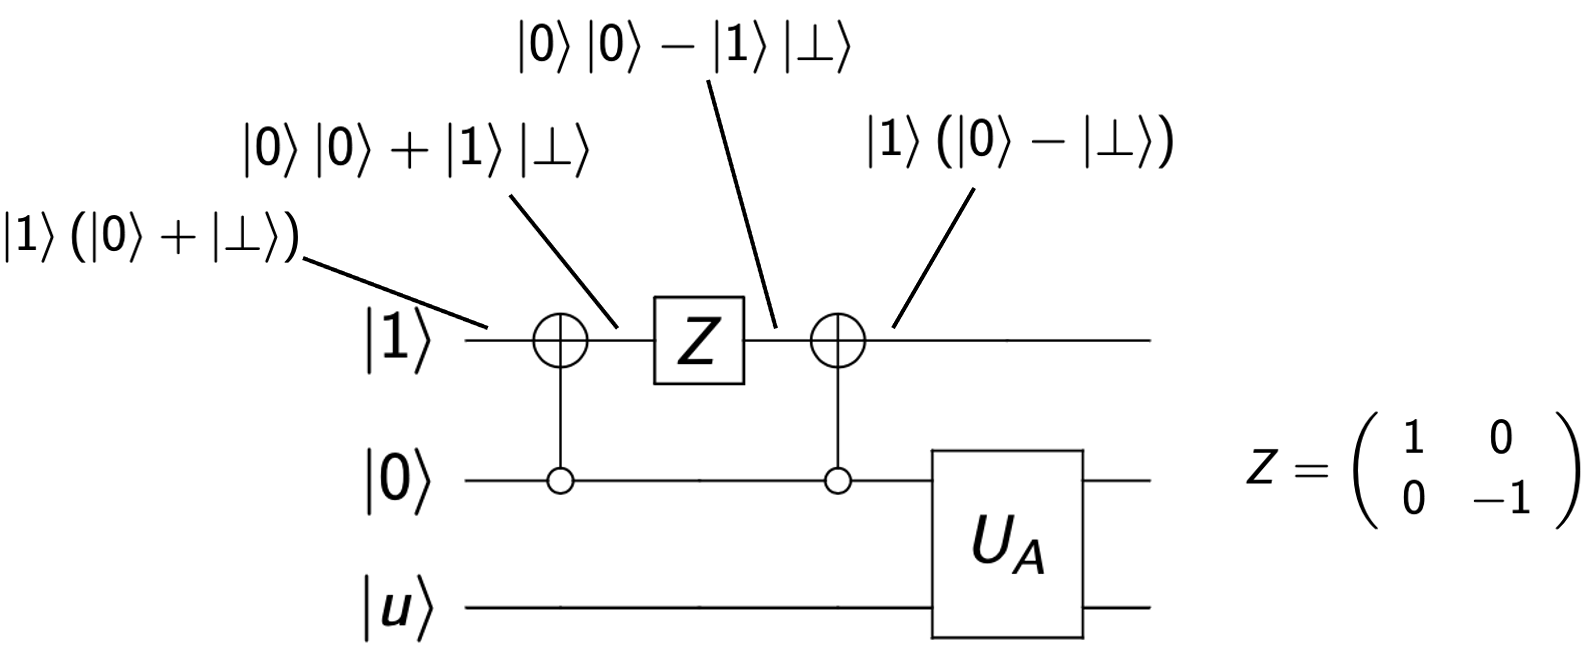
\includegraphics[width=0.85\textwidth]{images/page_30_img_1.png}

$U_A=\begin{pmatrix}A&*\\*&*\end{pmatrix}$, $U_A=U_A^\dagger$, $\Pi=\ket{0}\bra{0}\otimes I$, $Z_\Pi=2\Pi-I$
$$(U_A Z_\Pi)^k=\begin{pmatrix}T_k(A)&*\\*&*\end{pmatrix}$$
\end{frame}

\begin{frame}{Qubitization}
If $U_A$ is not Hermitian (but $A$ is): alternate between two 2D subspaces by applying $U_A$ and $U_A^\dagger$ alternately.

Circuit: $\ket{1}\xrightarrow{Z}\ket{0}\xrightarrow{U_A}\xrightarrow{U_A^\dagger}\cdots$
\end{frame}

\begin{frame}{Quantum signal processing (QSP)}
Starting from $2\times 2$ matrices $U(\lambda)$, $Z$, $O(\lambda)=U(\lambda)Z$, consider
$$U_\Phi(\lambda)=e^{i\phi_0 Z}\prod_{j=1}^{d}\bigl[O(\lambda)e^{i\phi_j Z}\bigr]
=\begin{pmatrix}P(\lambda)&-Q(\lambda)\sqrt{1-\lambda^2}\\Q^*(\lambda)\sqrt{1-\lambda^2}&P^*(\lambda)\end{pmatrix}$$
where $\Phi=(\phi_0,\phi_1,\ldots,\phi_d)\in\mathbb{R}^{d+1}$ are \emph{phase factors}.
\end{frame}

\begin{frame}{Quantum signal processing (QSP)}
\begin{block}{Theorem (QSP)}
Phase factors $\Phi\in\mathbb{R}^{d+1}$ exist such that $U_\Phi(\lambda)=\begin{pmatrix}P&*\\*&*\end{pmatrix}$
if and only if $P,Q$ satisfy:
\begin{enumerate}
\item $\deg P\le d$, $\deg Q\le d-1$,
\item $P$ has parity $d\bmod 2$; $Q$ has parity $(d-1)\bmod 2$,
\item $|P(\lambda)|^2+(1-\lambda^2)|Q(\lambda)|^2=1$ for all $\lambda\in[-1,1]$.
\end{enumerate}
\end{block}\footnote{[arXiv:1606.02685]}
\end{frame}

\begin{frame}{QSP + Qubitization}
The high-dimensional case follows via qubitization. Circuit:
\begin{align*}
\ket{1}&\xrightarrow{e^{i\tilde\phi_d Z}}\cdots\xrightarrow{e^{i\tilde\phi_0 Z}}\\
\ket{0}&\xrightarrow{U_A}\xrightarrow{U_A^\dagger}\cdots\xrightarrow{U_A^{(\dagger)}}\\
\ket{u}&\cdots
\end{align*}
Output: block-encoding of $P(A)$. \quad Query complexity: $d$.
\end{frame}

\begin{frame}{QSP for real polynomials}
\begin{block}{Theorem (QSP for real polynomials)}
Given a real polynomial $p(\lambda)$ with $\deg p=d$, $d\bmod 2$ parity, $|p(\lambda)|\le 1$ on $[-1,1]$, there exist $P,Q$ and phase factors $(\phi_0,\ldots,\phi_d)$ such that $\operatorname{Re}(P(\lambda))=p(\lambda)$ and
$$U_\Phi(\lambda)=\begin{pmatrix}P(\lambda)&*\\*&*\end{pmatrix}.$$
\end{block}
\end{frame}

\begin{frame}{QSP, qubitization, and QSVT}
For any Hermitian $A$ with $\|A\|\le1$ and block-encoding $U_A$, and any real polynomial $p$ of degree $d$ with $|p|\le1$ on $[-1,1]$:
$$p(A)\text{ can be block-encoded with }O(d)\text{ queries.}$$
If $A$ is not Hermitian, this becomes \textbf{singular value transformation (QSVT)}.\footnote{Gily\'{e}n et al.\ [arXiv:1806.01838]}
\end{frame}

\begin{frame}{Phase factors}
Finding phase factors was hard when QSP was proposed; now practically solved.
\begin{itemize}
\item \textbf{Direct methods:} Remez exchange, roots of polynomials [arXiv:1806.01838], Capitalization [arXiv:2003.02831], Prony's method [arXiv:2202.02671]
\item \textbf{Iterative methods:} optimization [arXiv:2002.11649], fixed-point iteration [arXiv:2209.10162], nonlinear Fourier transform [arXiv:2505.12615]
\end{itemize}
QSP reference: [arXiv:2510.00443]
\end{frame}

\section{Application: Hamiltonian simulation}
\begin{frame}\sectionpage\end{frame}

\begin{frame}{Hamiltonian simulation}
$$\frac{d}{dt}u(t)=-iHu(t),\quad 0\le t\le T,\quad H\text{ Hermitian}$$
\begin{itemize}
\item Unitary evolution: $e^{-iHt}$
\item A natural and promising application of quantum computers
\item Algorithms: product formula, quantum walk, truncated Taylor series, QSVT, randomization, \ldots
\end{itemize}
\end{frame}

\begin{frame}{QSVT for Hamiltonian simulation}
$U(T)=e^{-iHT}$. Consider $f(x)=e^{-ix\|H\|T}=\cos(\|H\|Tx)-i\sin(\|H\|Tx)$.

Polynomial approximations:
\begin{itemize}
\item Taylor: $\cos(\|H\|Tx)\approx\sum_{k=0}^{O(\|H\|T+\log(1/\epsilon))}\frac{(-1)^k\|H\|^{2k}T^{2k}}{(2k)!}x^{2k}$
\item Jacobi-Anger: $\cos(Tx)\approx J_0(\|H\|T)+2\sum_{k=1}^{O(\|H\|T+\log(1/\epsilon))}(-1)^kJ_{2k}(\|H\|T)T_{2k}(x)$
\end{itemize}
\end{frame}

\begin{frame}{QSVT for Hamiltonian simulation}
\textbf{Algorithm:} use QSVT to implement $\cos(TH)$ and $\sin(TH)$, then LCU to combine.

Query complexity:
$$O\!\left(\|H\|T+\log\tfrac{1}{\epsilon}\right)$$
\begin{itemize}
\item Optimal scaling
\item Drawback: cannot exploit structure inside $H=\sum_\gamma H_\gamma$, $H=-\Delta_x+V(x)$
\end{itemize}
\end{frame}

\begin{frame}{Product formula}
$H=A+B$. Split evolution:
$$e^{-iHT}=\lim_{L\to\infty}\left(e^{-iBT/L}e^{-iAT/L}\right)^L$$
\begin{itemize}
\item 1st order: $U_1(t)=e^{-iBt}e^{-iAt}\approx e^{-iHt}+O(t^2)$
\item 2nd order: $U_2(t)=e^{-iAt/2}e^{-iBt}e^{-iAt/2}\approx e^{-iHt}+O(t^3)$
\item Suzuki recursion: $U_{2p+2}(t)=U_{2p}(s_pt)^2U_{2p}((1-4s_p)t)U_{2p}(s_pt)^2$
\end{itemize}
Complexity (commutator scaling, suboptimal in $T,\epsilon$):
$$O\!\left(\frac{\alpha_{\mathrm{comm}}^{1/p}T^{1+1/p}}{\epsilon^{1/p}}\right)$$
\end{frame}

\begin{frame}{Multi-product formula}
Simultaneously achieve commutator scaling and optimal time/precision via extrapolation:
$$U_{\mathrm{MPF}}(t)=\sum_{j=1}^M a_j U_2(t/k_j)^{k_j}$$
\end{frame}

\begin{frame}{Time-dependent Hamiltonian simulation}
$$\frac{d}{dt}u(t)=-iH(t)u(t),\quad 0\le t\le T,\quad H(t)\text{ Hermitian}$$
\begin{itemize}
\item Product formula: commutator scaling (including derivatives), suboptimal in $T,\epsilon$
\item Truncated Dyson series: near-optimal
$$O\!\left(\max_t\|H(t)\|T\log\frac{\max_t\|H(t)\|T}{\epsilon}\right)$$
\end{itemize}
Reference: [arXiv:2411.03180]
\end{frame}

\section{Application: Linear systems of equations}
\begin{frame}\sectionpage\end{frame}

\begin{frame}{Quantum linear system problem (QLSP)}
\textbf{Classical:} given $N\times N$ Hermitian $A$ and vector $b$, compute $x=A^{-1}b$.

Non-Hermitian: embed as $\begin{pmatrix}0&A\\A^\dagger&0\end{pmatrix}\begin{pmatrix}0\\x\end{pmatrix}=\begin{pmatrix}b\\0\end{pmatrix}$.

\textbf{Quantum:} find $\epsilon$-approximation of $\ket{x}=\frac{A^{-1}\ket{b}}{\|A^{-1}\ket{b}\|}$.

Key parameters: error $\epsilon$, condition number $\kappa=\|A\|\|A^{-1}\|$.
\end{frame}

\begin{frame}{QSVT for QLSP}
$A=W\Sigma V^\dagger\to A^{-1}=V\Sigma^{-1}W^\dagger$. Consider $f(x)=\frac{1}{\kappa x}$.

Polynomial approx: odd polynomial $p(x)$ of degree $O(\kappa\log(1/\epsilon))$ with $|p|\le1$ and $|p(x)-1/(\kappa x)|\le\epsilon$ for $x\in[1/\kappa,1]$.

\textbf{Algorithm:} QSVT to implement $p(A^\dagger)$, apply to $\ket{0}\ket{b}$, post-select.
\end{frame}

\begin{frame}{Harrow-Hassidim-Lloyd (HHL)}
The first quantum algorithm for QLSP.\footnote{[arXiv:0811.3171]}

Let $(\lambda_j,\ket{v_j})$ be eigenpairs of $A$ and $\ket{b}=\sum_j\beta_j\ket{v_j}$:
$$A^{-1}\ket{b}=\left(\sum_j\lambda_j^{-1}\ket{v_j}\bra{v_j}\right)\left(\sum_j\beta_j\ket{v_j}\right)=\sum_j\frac{\beta_j}{\lambda_j}\ket{v_j}$$
Subroutines:
\begin{itemize}
\item \textbf{QPE:} $U_{\mathrm{QPE}}\ket{\psi}\ket{0}=\ket{\psi}\ket{\theta}$ where $U\ket{\psi}=e^{2\pi i\theta}\ket{\psi}$
\item \textbf{Controlled rotation:} $U_{\mathrm{CR}}\ket{\theta}\ket{0}=\ket{\theta}\bigl(f(\theta)\ket{0}+\cdots\bigr)$
\end{itemize}
\end{frame}

\begin{frame}{HHL}
\centering
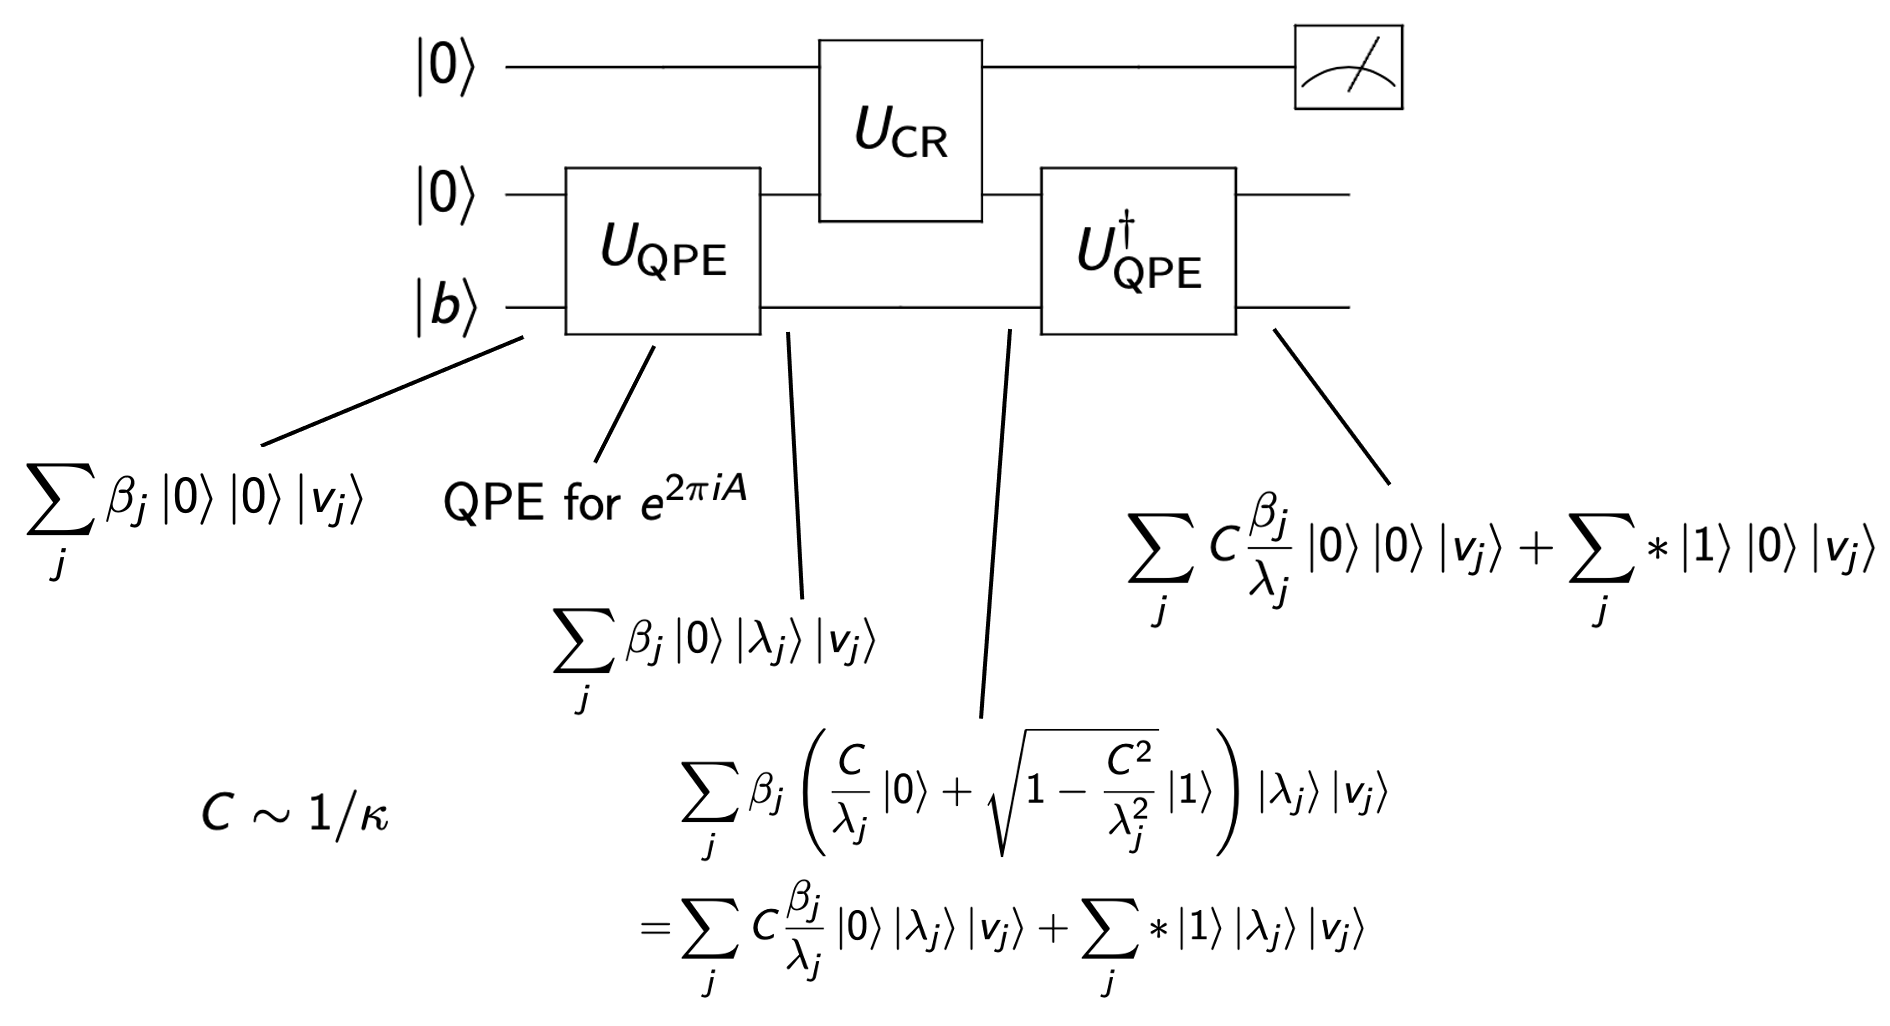
\includegraphics[width=0.85\textwidth]{images/page_49_img_1.png}
\end{frame}

\begin{frame}{LCU: Fourier approach}
Key identity: $\dfrac{1}{x}=\dfrac{i}{\sqrt{2\pi}}\int_0^\infty dy\int_{-\infty}^\infty dz\,ze^{-z^2/2}e^{-ixyz}$.

For Hermitian $A$:
$$A^{-1}\approx\sum_{j,j'}c_{j,j'}e^{-iy_jz_{j'}A}$$
implemented by LCU + Hamiltonian simulation.
\end{frame}

\begin{frame}{Adiabatic Quantum Computing (AQC)}
\begin{columns}
\begin{column}{0.55\textwidth}
$$i\partial_t\ket{\psi(t)}=H(t/T)\ket{\psi(t)},\quad t\in[0,T]$$
\begin{itemize}
\item Eigenvector of $H(0)\to$ eigenvector of $H(1)$ if $T$ large enough and gap condition holds
\item Application: quantum computing model for eigenvalue problems
\end{itemize}
\end{column}
\begin{column}{0.42\textwidth}
\centering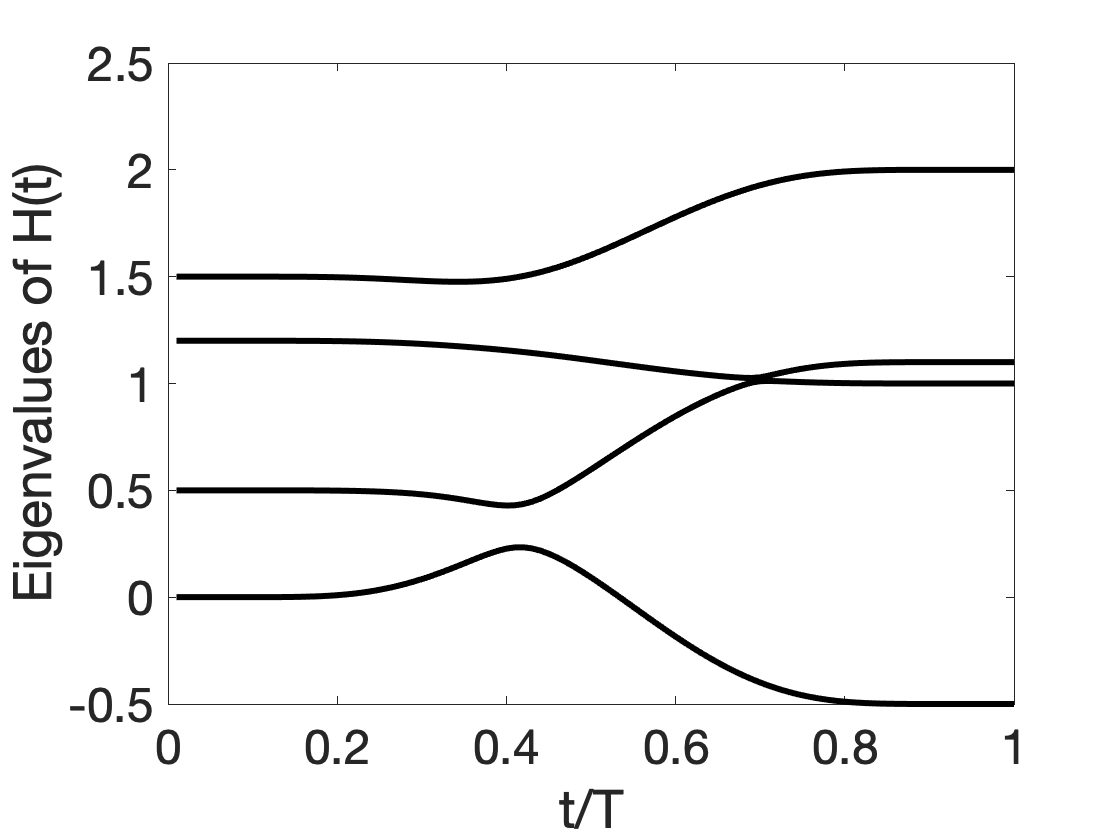
\includegraphics[width=\textwidth]{images/page_51_img_1.png}
\end{column}
\end{columns}
\end{frame}

\begin{frame}{AQC for QLSP}
$$H_0=\begin{pmatrix}0&Q_b\\Q_b&0\end{pmatrix},\quad H_1=\begin{pmatrix}0&AQ_b\\Q_bA&0\end{pmatrix},\quad Q_b=I-\ket{b}\bra{b}$$
$$H(s)=(1-f(s))H_0+f(s)H_1$$
\begin{itemize}
\item Eigenpath at eigenvalue 0 connects $[b;0]$ and $[x;0]$
\item Need to carefully choose scheduling function $f(s)$
\end{itemize}
\end{frame}

\begin{frame}{Complexities}
\centering\small
\begin{tabular}{lcc}
\toprule
Method & Circuit ($A$) & Circuit ($b$)\\
\midrule
HHL [0811.3171] & $O(\kappa^2/\epsilon)$ & $O(\kappa)$\\
LCU [1511.02306] & $O(\kappa^2\mathrm{polylog}(\kappa/\epsilon))$ & $O(\kappa)$\\
QSVT [1804.01973] & $O(\kappa^2\log(\kappa/\epsilon))$ & $O(\kappa)$\\
RM [1805.10549] & $O((\kappa/\epsilon)\log\kappa)$ & $O((\kappa/\epsilon)\log\kappa)$\\
AQC($p$) [1909.05500] & $O((\kappa/\epsilon)\log(\kappa/\epsilon))$ & $O((\kappa/\epsilon)\log(\kappa/\epsilon))$\\
AQC(exp) [1909.05500] & $O(\kappa\,\mathrm{polylog}(\kappa/\epsilon))$ & $O(\kappa\,\mathrm{polylog}(\kappa/\epsilon))$\\
dAQC+EF [2111.08152] & $O(\kappa\log(1/\epsilon))$ & $O(\kappa\log(1/\epsilon))$\\
KR [2406.12086] & $O(\kappa\log(1/\epsilon))$ & $O(\kappa\log(1/\epsilon))$\\
Tunable VTAA [2410.18178] & $O(\kappa\log(\kappa/\epsilon)\log(1/\epsilon))$ & $O(\kappa)$\\
\bottomrule
\end{tabular}
\end{frame}

\section{Summary}
\begin{frame}\sectionpage\end{frame}

\begin{frame}{Summary}
\textbf{Quantum computing:} use quantum mechanics to perform computing.

\textbf{Input models:} Vector: quantum state \quad Matrix: block-encoding

\textbf{Algorithms:}
\begin{itemize}
\item LCU
\item Matrix functions: QSVT can implement degree-$d$ polynomials with cost $O(d)$
\item Hamiltonian simulation: QSVT, product formula
\item Linear systems: QSVT, HHL, LCU, adiabatic
\end{itemize}
\end{frame}

\begin{frame}{Additional resources}
\begin{itemize}
\item IPAM Tutorial: Mathematical and Computational Challenges in Quantum Computing (Sept.\ 12--15, 2023)\\
{\small\url{https://www.ipam.ucla.edu/programs/workshops/}\\\url{mathematical-and-computational-challenges-in-quantum-computing-tutorials/}}
\item Lecture notes by Lin Lin:\\
\url{https://math.berkeley.edu/~linlin/qasc/}
\end{itemize}
\vspace{1em}
\centering\Large Thank you!\\[4pt]\normalsize\texttt{dongan@pku.edu.cn}
\end{frame}

%% -------------------------------------------------------
%% Appendix
%% -------------------------------------------------------
\appendix

\begin{frame}{Matrix addition}
Goal: block-encode $\sum_j c_j A_j$ for $\|A_j\|\le1$.

Algorithm: LCU with $U_{A_j}$ as block-encodings.
$$O_s=\sum_j\ket{j}\bra{j}\otimes U_{A_j},\qquad U_{A_j}=\begin{pmatrix}A_j&*\\*&*\end{pmatrix}$$
\end{frame}

\begin{frame}{Vector addition}
Goal: compute $\sum_j c_j\ket{u_j}$.

Algorithm: LCU with state prep oracles $U_j:\ket{0}\to\ket{u_j}$:
$$\sum_j c_jU_j\ket{0}=\sum_j c_j\ket{u_j}$$
\end{frame}

\begin{frame}{Matrix multiplication}
Two block-encodings $U_{A_0}$, $U_{A_1}$. Naïve stacking does \emph{not} work:
$$U_{A_1}U_{A_0}\ket{0}\ket{u_0}\ne\ket{0}A_1A_0\ket{u_0}+\cdots$$
\textbf{Method 1: duplicate ancilla qubits.} Multiplication of $J$ matrices uses $O(J)$ extra ancilla qubits.
\end{frame}

\begin{frame}{Matrix multiplication}
\textbf{Method 2: compression gadget}\\
(Low-Wiebe [arXiv:1805.00675]; Fang-Lin-Tong [arXiv:2208.06941])
\centering
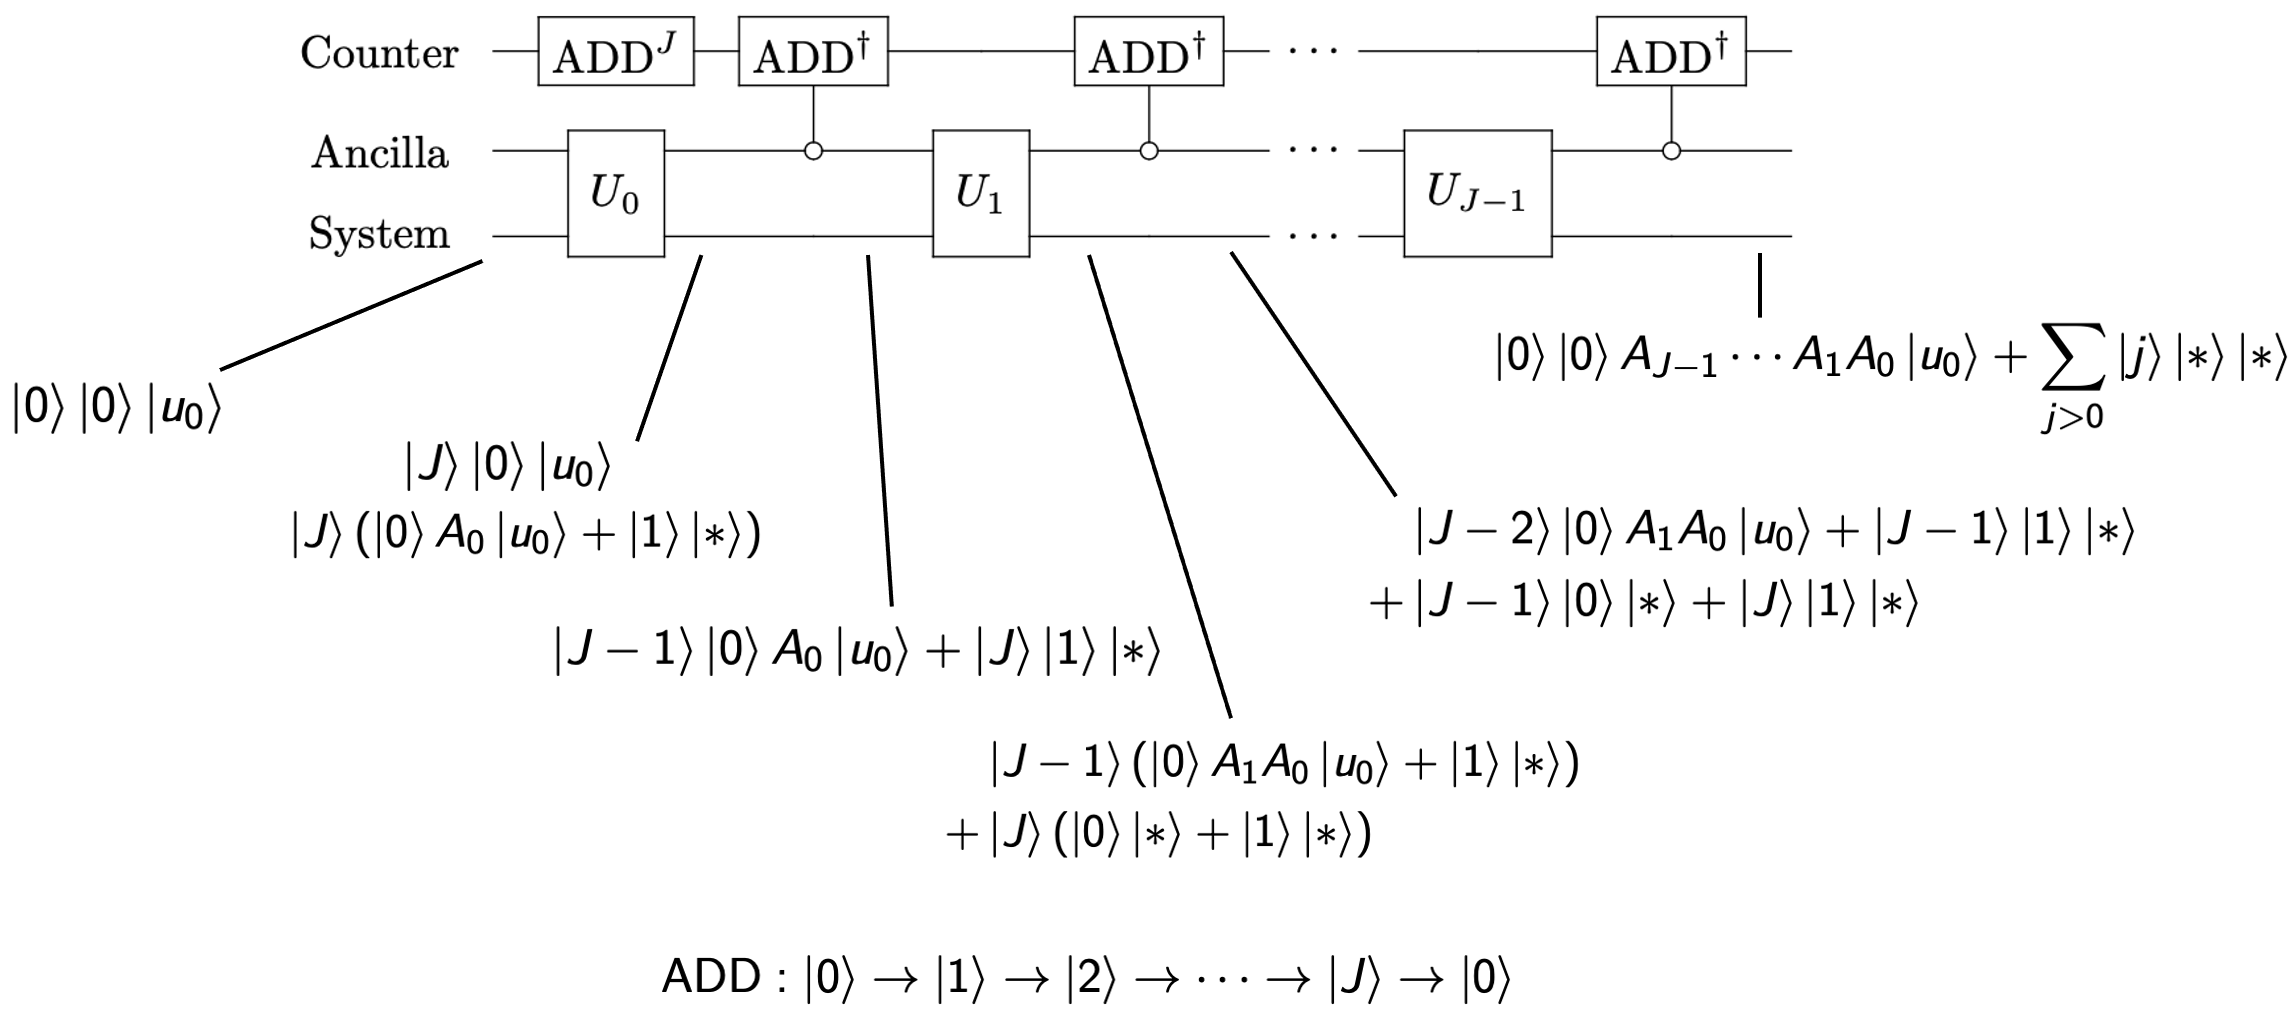
\includegraphics[width=0.82\textwidth]{images/page_61_img_1.png}
\end{frame}

\begin{frame}{Qubitization (non-Hermitian block-encoding)}
For general (non-Hermitian) $U_A$:
$$U_A\ket{0}\ket{v_j}=\lambda_j\ket{0}\ket{v_j}+\sqrt{1-\lambda_j^2}\ket{\perp'_j},\qquad
U_A^\dagger\ket{0}\ket{v_j}=\lambda_j\ket{0}\ket{v_j}+\sqrt{1-\lambda_j^2}\ket{\perp_j}$$
$$[U_A]_{\mathcal{H}_j\to\mathcal{H}'_j}=[U_A^\dagger]_{\mathcal{H}'_j\to\mathcal{H}_j}=\begin{pmatrix}\lambda_j&\sqrt{1-\lambda_j^2}\\\sqrt{1-\lambda_j^2}&-\lambda_j\end{pmatrix}$$
$$(U_A^\dagger Z_\Pi U_A Z_\Pi)^k=\begin{pmatrix}T_{2k}(A)&*\\*&*\end{pmatrix}$$
\end{frame}

\begin{frame}{Quantum signal processing (QSP)}
$$U_\Phi(\lambda)=e^{i\phi_0 Z}\prod_{j=1}^d\bigl[U(\lambda)e^{i\phi_j Z}\bigr]=\begin{pmatrix}P(\lambda)&*\\*&*\end{pmatrix}$$
Using $Ze^{i\phi Z}=(-i)e^{i(\phi+\pi/2)Z}$, we can absorb $Z$ into modified phases:
\begin{itemize}
\item Even $d$: $\tilde\phi_j=\phi_j+(-1)^j\pi/2$ for $j\ne0$; $\tilde\phi_0=\phi_0$
\item Odd $d$: same, with an extra $Z$ that doesn't affect the top-left element
\end{itemize}
\end{frame}

\begin{frame}{QSP + Qubitization}
For Hermitian $A$ and polynomial $P(x)$ satisfying QSP conditions:
\begin{itemize}
\item Even $d$: $e^{i\tilde\phi_0 Z_\Pi}\prod_{j=1}^{d/2}\bigl[U_A^\dagger e^{i\tilde\phi_{2j-1}Z_\Pi}U_A e^{i\tilde\phi_{2j}Z_\Pi}\bigr]=\begin{pmatrix}P(A)&*\\*&*\end{pmatrix}$
\item Odd $d$: similar with alternating $U_A$, $U_A^\dagger$
\end{itemize}
\end{frame}

\begin{frame}{QSP/QSVT vs LCU}
\begin{columns}
\begin{column}{0.55\textwidth}
\begin{itemize}
\item Both can implement matrix functions
\item LCU has overhead from $\ell^1$-norm of coefficients and extra control logic
\item For general matrices:
\begin{itemize}
\item QSVT: singular value transformation
\item LCU: eigenvalue transformation via $f(A)=\frac{1}{2\pi i}\oint_\Gamma f(z)(z-A)^{-1}dz$
\end{itemize}
\end{itemize}
\end{column}
\begin{column}{0.42\textwidth}
\centering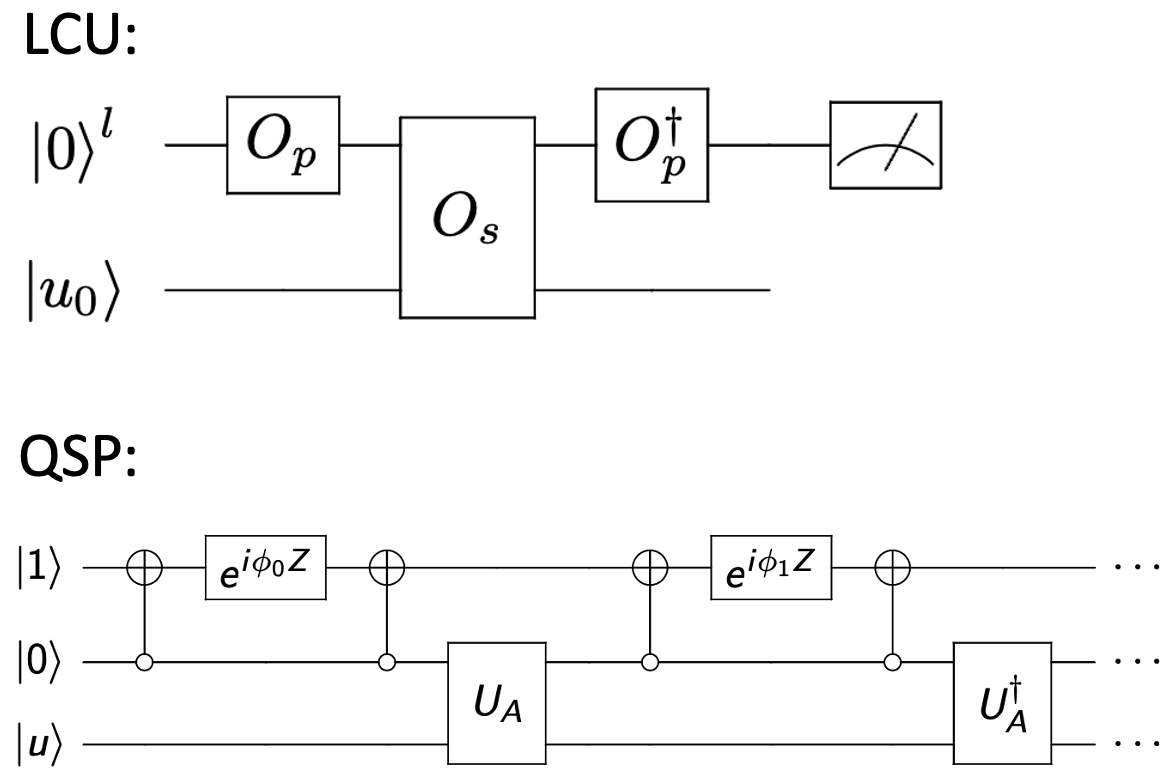
\includegraphics[width=\textwidth]{images/page_68_img_1.png}
\end{column}
\end{columns}
\end{frame}

\begin{frame}{HHL: complexity}
Two sources:
\begin{itemize}
\item Cost per run (mainly QPE): $O(\kappa/\epsilon)$
\item Number of repeats: $O(1/(C\|A^{-1}\ket{b}\|))=O(\kappa)$
\item Overall: $O(\kappa^2/\epsilon)$
\end{itemize}
Subroutines needed: Hamiltonian simulation ($e^{2\pi iA}$) and QPE.
\end{frame}

\begin{frame}{LCU: Chebyshev approach}
\begin{columns}
\begin{column}{0.55\textwidth}
Expand $1/x$ in Chebyshev polynomials:
$$A^{-1}\approx\sum_{j=0}^{O(\kappa\,\mathrm{polylog}(\kappa/\epsilon))}c_j T_{2j+1}(A)$$
$\|T_{2j+1}(A)\|\le1$ but not unitary $\Rightarrow$ need block-encoding.

Same overall complexity: $\kappa\,\mathrm{polylog}(\kappa/\epsilon)\times\kappa/\sqrt{\log(\kappa/\epsilon)}=O(\kappa^2\,\mathrm{polylog}(\kappa/\epsilon))$.
\end{column}
\begin{column}{0.42\textwidth}
\centering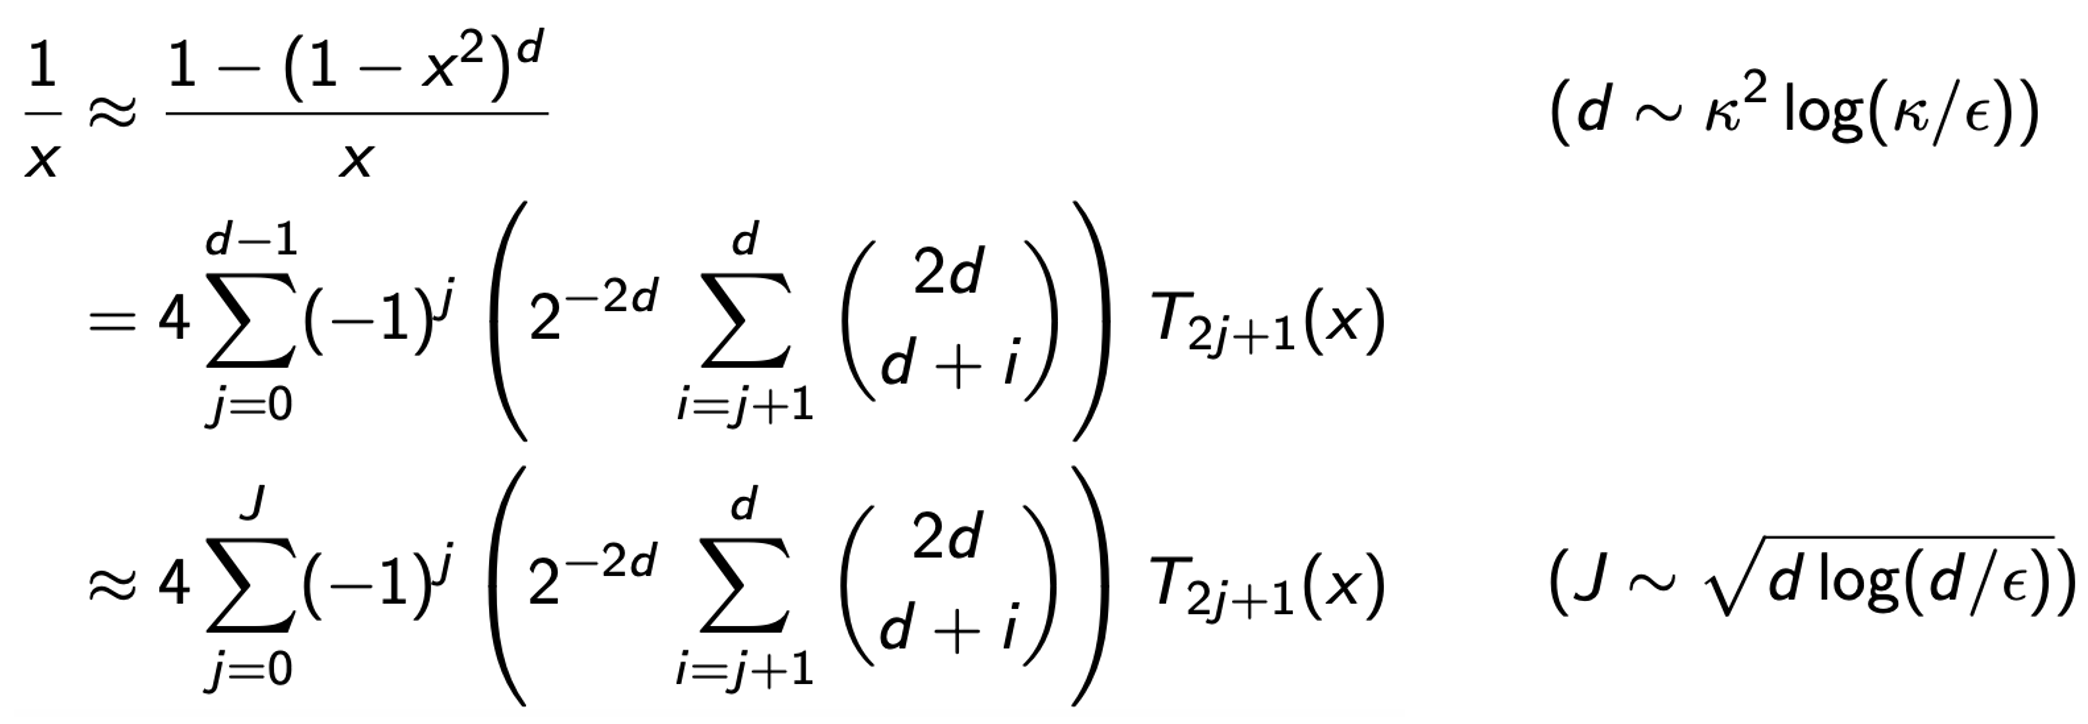
\includegraphics[width=\textwidth]{images/page_70_img_1.png}
\end{column}
\end{columns}
\end{frame}

\begin{frame}{HHL circuit}
\centering
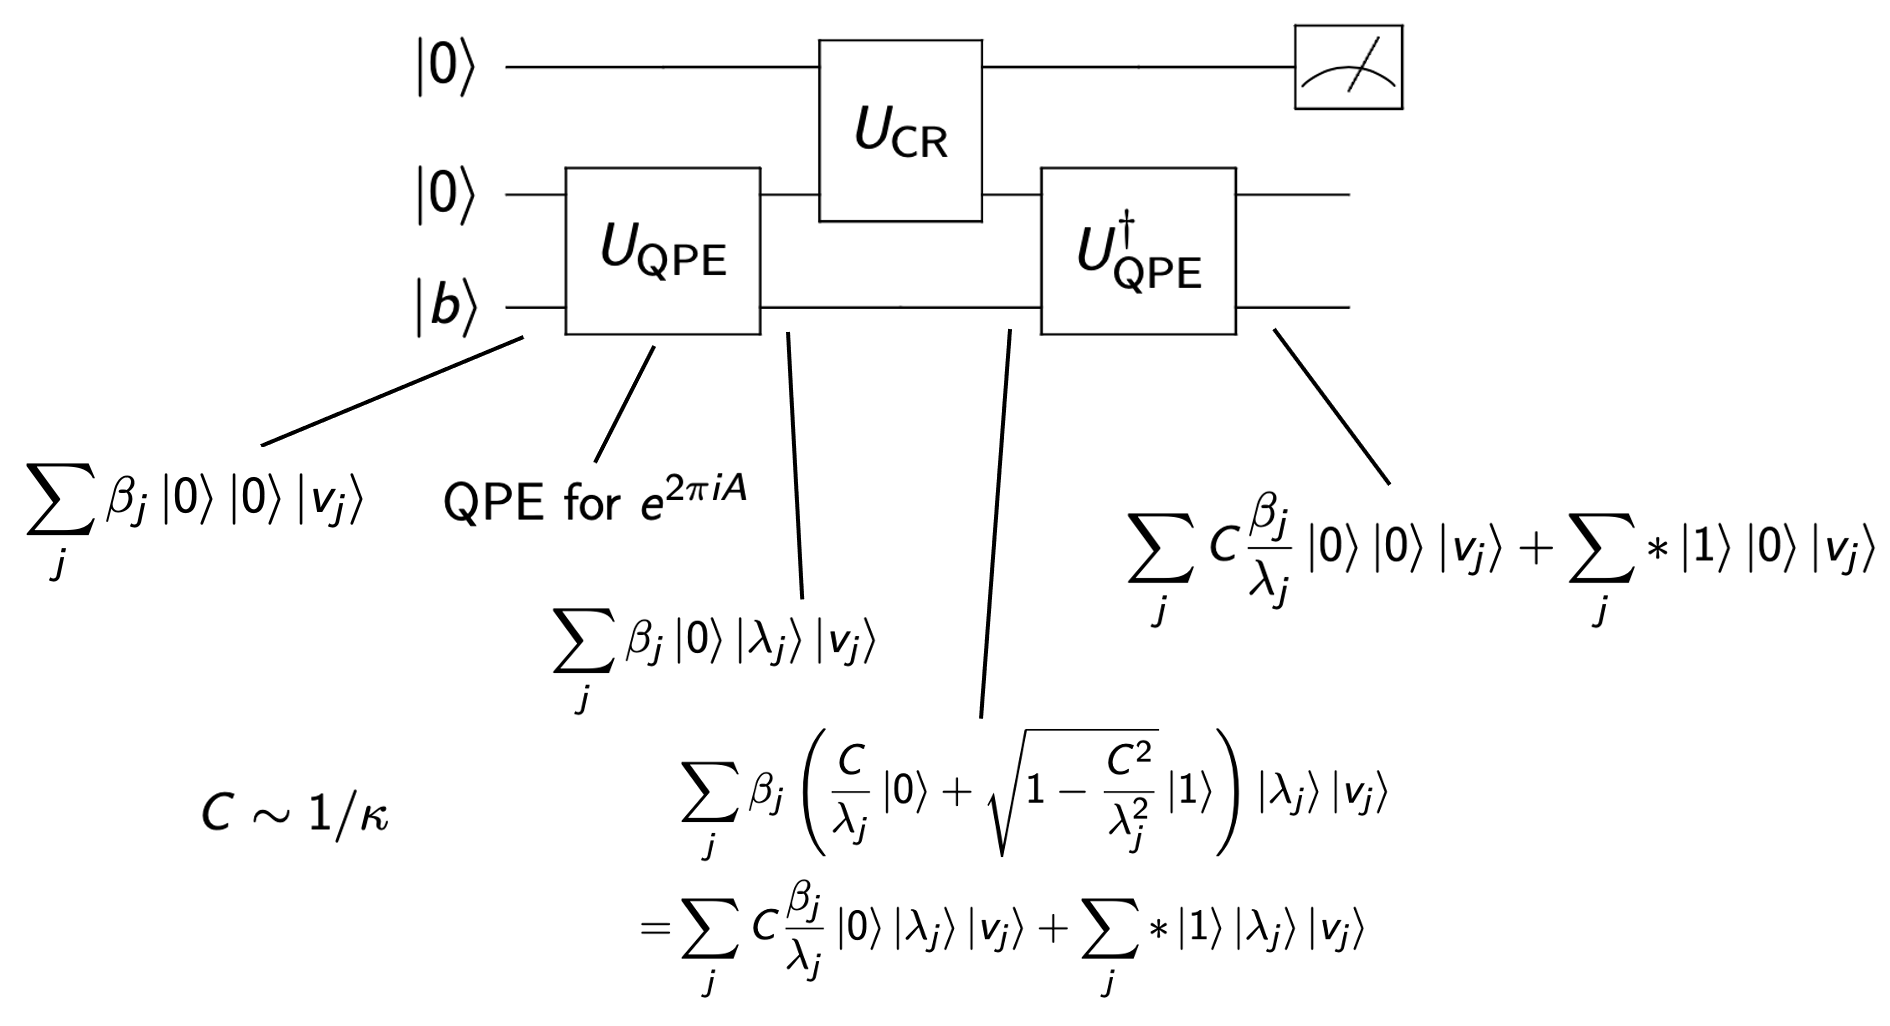
\includegraphics[width=0.85\textwidth]{images/page_74_img_1.png}
\end{frame}

\begin{frame}{Quantum Adiabatic Theorem}
\begin{block}{Theorem (Jansen-Ruskai-Seiler)}
With gap $\Delta(s)$:
$$\eta(s)\le C\left\{\frac{\|H'(0)\|^2}{T\Delta^2(0)}+\frac{\|H'(s)\|^2}{T\Delta^2(s)}+\frac{1}{T}\int_0^s\left(\frac{\|H''(\tau)\|^2}{\Delta^2(\tau)}+\frac{\|H'(\tau)\|^4}{\Delta^3(\tau)}\right)d\tau\right\}$$
\end{block}
\begin{itemize}
\item Error $\le\epsilon$: $T=O(\Delta_*^{-3}\epsilon^{-1})$ — cubic dependence on gap
\item In QLSP: $\Delta_*\sim1/\kappa\Rightarrow T=O(\kappa^3\epsilon^{-1})$
\end{itemize}
\end{frame}

\begin{frame}{Time-optimal AQC}
Interpolate $H(s)=(1-f(s))H_0+f(s)H_1$; choose $f(s)$ to slow down when gap is small.

$\text{AQC}(p)$: $\dot f(s)=c\,\Delta^p(f(s))\Rightarrow T=O(\kappa/\epsilon)$.\footnote{An-Lin [arXiv:1909.05500]}
\end{frame}

\begin{frame}{AQC(exp)}
Improved adiabatic theorem: error $\sim O(T^{-k})$ with boundary cancellation.

$\text{AQC(exp)}$: $f(s)=c^{-1}\int_0^s\exp[-u^{-1}(1-u)^{-1}]du\Rightarrow T=O(\kappa\,\mathrm{polylog}(\kappa/\epsilon))$.\footnote{An-Lin [arXiv:1909.05500]}
\end{frame}

\begin{frame}{Preconditioning}
$\mathcal{A}x=b\Leftrightarrow M\mathcal{A}x=Mb$; effective if $\kappa(M\mathcal{A})\ll\kappa(\mathcal{A})$.

Classical: diagonal, incomplete factorization, SPAI, \ldots

Quantum: SPAI [arXiv:1301.2340], circulant [Shao-Xiang].
\end{frame}

\begin{frame}{Preconditioning: $(A+B)\ket{x}\approx\ket{b}$}
Assume $A$ easily invertible, large $\|A\|$, moderate $\|B\|,\|A^{-1}\|,\|(A+B)^{-1}\|$.

$\kappa(A+B)\sim O(\|A\|)$. Preconditioner $A^{-1}$: $\kappa(I+A^{-1}B)=O(1)$.

Algorithm pipeline:
$$A^{-1}\to A^{-1}B\to I+A^{-1}B\to(I+A^{-1}B)^{-1}\to(I+A^{-1}B)^{-1}A^{-1}=(A+B)^{-1}$$
Needs: matrix addition, multiplication, and fast inversion of a diagonal matrix.
\end{frame}

\end{document}

